%!TEX root = ../thesis.tex
%*******************************************************************************
%*********************************** Analysis Overview *********
%*******************************************************************************

\chapter{Simplified likelihoods}\label{ch:simplify}

\ifpdf
    \graphicspath{{chapter-simplify/Figs/Raster/}{chapter-simplify/Figs/PDF/}{chapter-simplify/Figs/}}
\else
    \graphicspath{{chapter-simplify/Figs/Vector/}{chapter-simplify/Figs/}}
\fi

In the previous chapter, the concept of preserving an analysis for the purpose of reinterpretations has been introduced, and an example of a fully preserved analysis pipeline using containerised workflows has been discussed. In large-scale reinterpretations involving a large number of \gls{susy} models to be tested against, the wall time needed for statistical inference can be a computational bottleneck and thus calls for simplifications of the statistical model of an analysis. This chapter therefore introduces the concept of \textit{simplified likelihoods} as approach to approximate the statistical model of an analysis.

\section{Motivation}\label{sec:simplified_likelihood_motivation}

Reinterpretations of ATLAS SUSY searches in more complete and realistic \gls{susy} scenarios (as opposed to simplified models) often involves high-dimensional parameter spaces that are computationally extremely challenging to sample and compare to ATLAS data in an exhaustive way. Large-scale reinterpretations of this type have already been performed in ATLAS after the Run~1 data-taking period in both the 19-dimensional \gls{pmssm}~\cite{SUSY-2014-08} (introduced in~\cref{sec:theory_pmssm}) as well as a 5-dimensional representation of the \gls{pmssm}~\cite{Aaboud:2016wna}. Due to the complexity of the statistical models of today's SUSY searches in ATLAS, originating from the large number of channels and the large amount of nuisance parameters typically considered, the wall time needed for the statistical inference is usually far from negligible. In a typical large-scale reinterpretation involving $\mathcal{O}(10^5-10^6)$ sampled models, an optimistic estimation of the wall time needed for the statistical inference per model of $\mathcal{O}(\SI{10}{\second}-\SI{e2}{\second})$ is too computationally expensive, especially when more than just a few ATLAS \gls{susy} searches are included.

One approach of alleviating this computational problem is to approximate the \gls{susy} searches through their model-independent limits published in conjunction with the model-dependent exclusion limits. By construction, the model-independent limits are derived using only cut-and-count signal regions without multi-bin or shape-fit setups, thus making minimal model assumptions. While computationally very fast, this approach naturally underestimates the true exclusion power of the respective analysis due to the fact that model-dependent properties are not exploited (as they typically are in the exclusion signal regions). \Cref{fig:single_bin} compares the exclusion contours obtained with the full set of exclusion signal regions (shown in orange) to the exclusion contours obtained using the discovery signal regions (shown in green), defined in~\cref{tab:SignalRegionDef}. As the discovery signal regions are not mutually exclusive, they are not statistically combined and thus three separate observed and expected contours can be drawn. From \cref{fig:single_bin}, it is clear that even a best-expected combination of the three discovery signal regions does not reach the sensitivity achieved using the two-dimensional shape-fit setup resulting from statistical combination of the nine exclusion signal regions. Nonetheless, this approach has been opted for in the large-scale scan of the \gls{pmssm} using ATLAS data from Run~1~\cite{SUSY-2014-08}, yielding conservative exclusion power and thus room for improvement.

Therefore, the following sections introduce a method for approximating ATLAS SUSY searches without disregarding their elaborate use of multi-bin signal regions exploiting the varying shapes of signal and \gls{sm} background distributions. 

\begin{figure}
	\centering
	\begin{subfigure}[b]{0.5\textwidth}
		\centering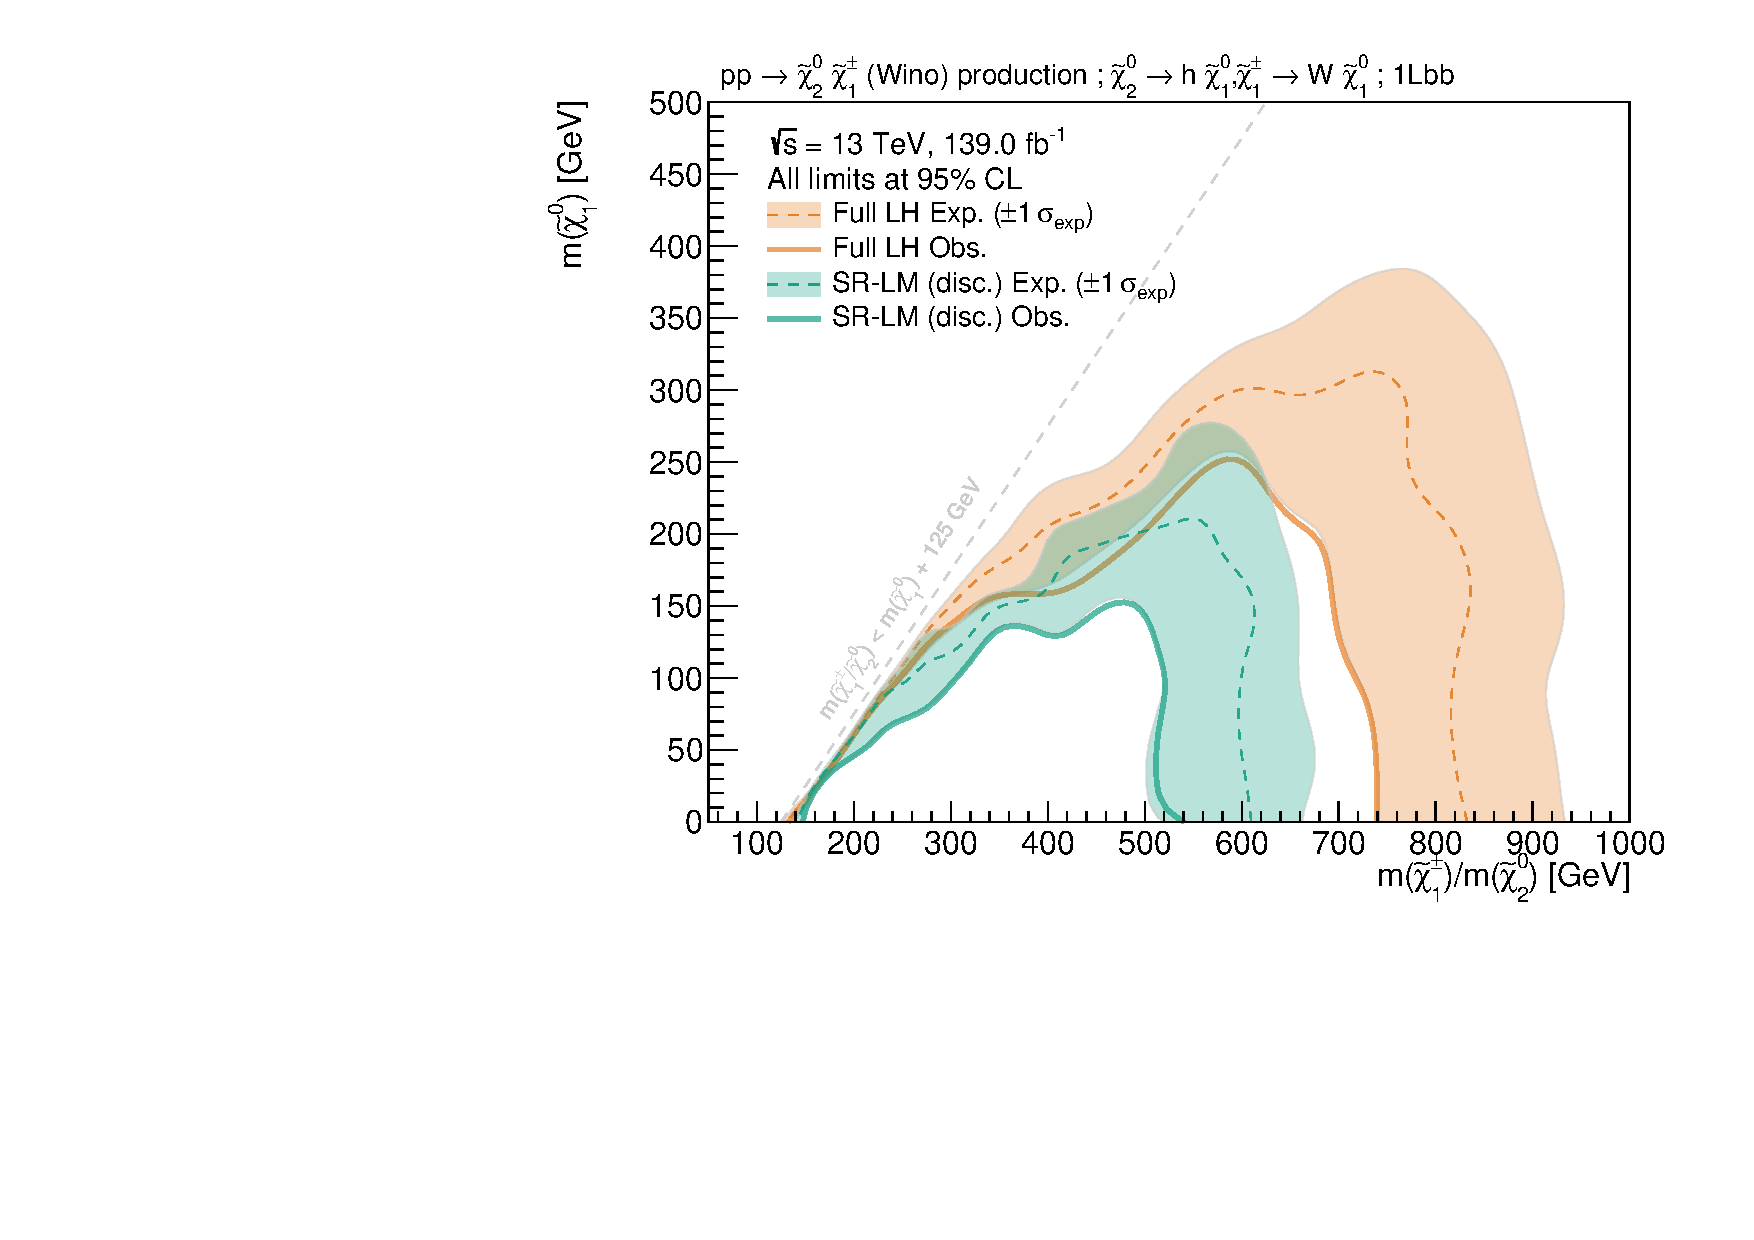
\includegraphics[width=\textwidth]{exclusion_1Lbb_SRLM_noLabel}
		\caption{Discovery SR-LM\label{fig:single_bin_SRLM}}
	\end{subfigure}\hfill
	\begin{subfigure}[b]{0.5\textwidth}
		\centering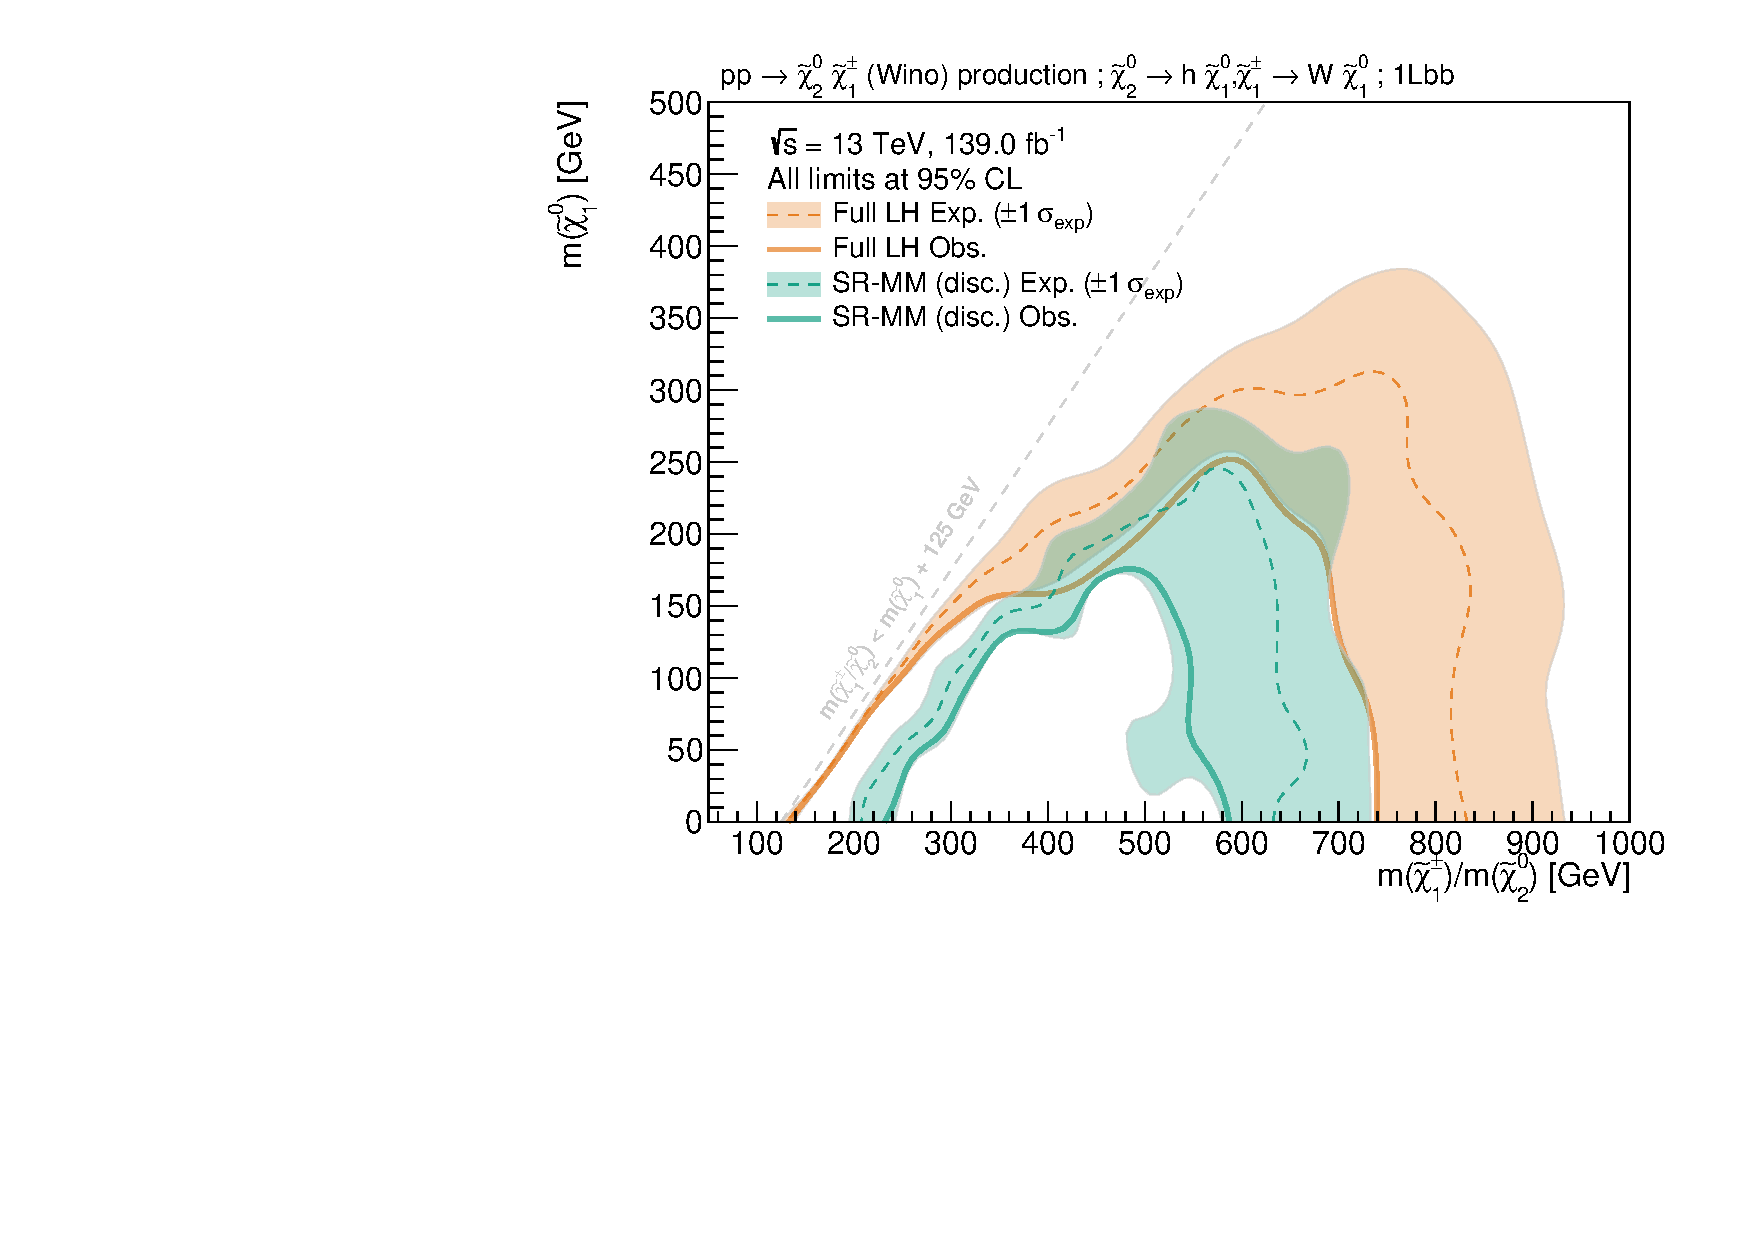
\includegraphics[width=\textwidth]{exclusion_1Lbb_SRMM_noLabel}
		\caption{Discovery SR-MM\label{fig:single_bin_SRMM}}
	\end{subfigure}\hfill
	\begin{subfigure}[b]{0.5\textwidth}
		\centering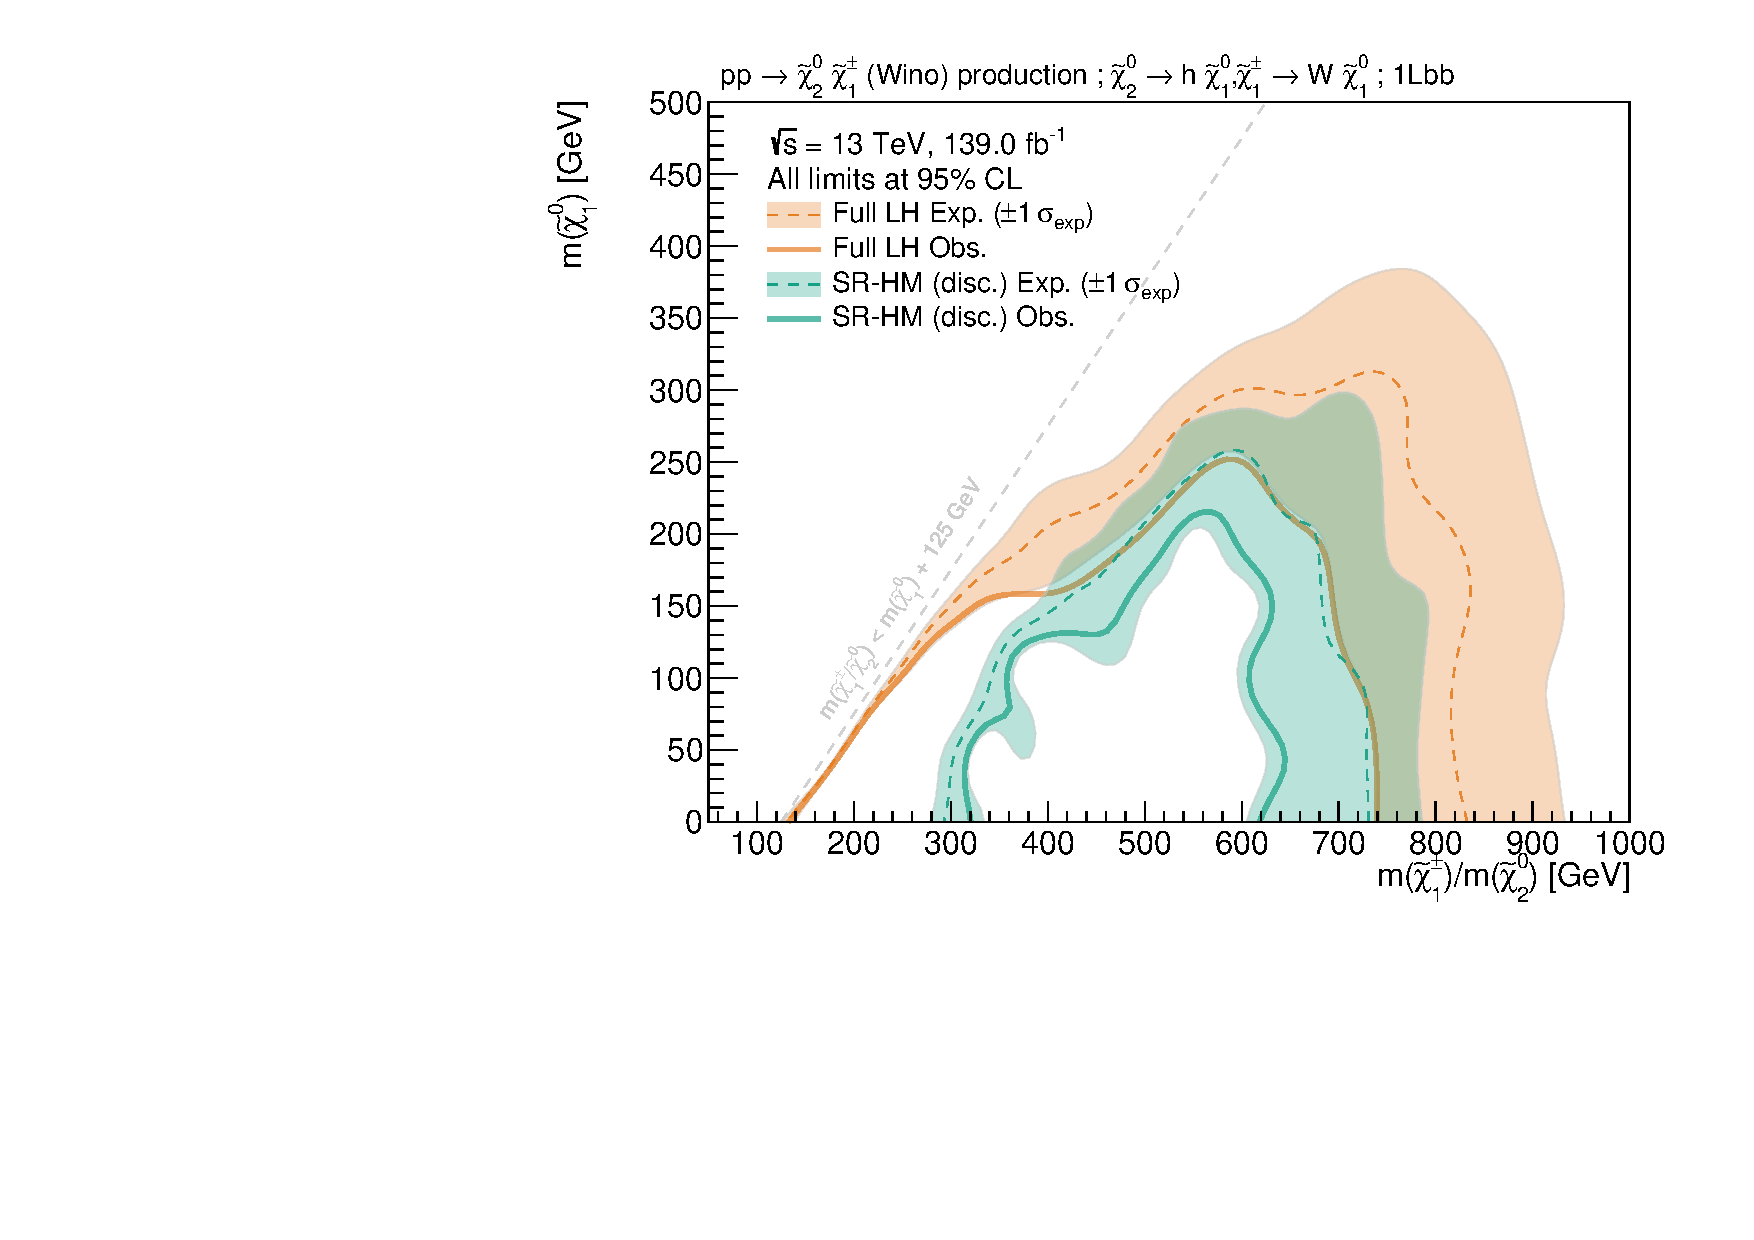
\includegraphics[width=\textwidth]{exclusion_1Lbb_SRHM_noLabel}
		\caption{Discovery SR-HM\label{fig:single_bin_SRHM}}
	\end{subfigure}%
	\caption{Comparison of exclusion limits obtained using a likelihood built from all nine exclusion signal regions (orange), and the discovery signal regions (green). As discussed in~\cref{sec:signal_region_definitions}, the discovery signal regions are simple cut-and-count regions with minimal model assumptions. They are not mutually exclusive, they cannot be fitted together, thus resulting in three separate exclusion contours. All statistical and systematic uncertainties on the background and the signal event rates are included.}\label{fig:single_bin}
\end{figure}

\section{Building simplified likelihoods}\label{sec:building_simplified_likelihoods}



In order to retain the full statistical combination of multiple signal region bins implemented in many SUSY searches, while still being able to achieve a sufficiently fast approximation, the statistical treatment of the systematic uncertainties as well as of the background model needs to be simplified. In the procedure presented in the following, this is achieved by first performing a background-only fit to data in all \glspl{sr} and \glspl{cr}, in order to determine the best-fit values of all the model parameters $\boldsymbol{\phi}$. This allows to determine the post-fit total background rate estimate as well as the total uncertainty on that estimate in every bin. 

As the full likelihood in \texttt{JSON} format defines the full statistical model used for statistical inference in the analysis, the above background-only fit can be performed using \texttt{pyhf} and the preserved full likelihood of the analysis. With the full likelihoods starting to become available on \textsc{HEPData} (see \eg \reference\cite{fullLH_1Lbb}) this procedure can rely on public information only. The simplified likelihoods introduced in the following, follow the same likelihood \texttt{JSON} specification introduced for the full likelihoods in \reference\cite{ATL-PHYS-PUB-2019-029}. The following description only highlights the specification details relevant to the simplified likelihood. 

In the simplified likelihood, the background model is approximated with a single background sample, representing the total \gls{sm} background rate in the different analysis channels (called \texttt{total\_bkg} in \cref{lst:bkg_sample}). The sample rate of the total background sample is set to the total post-fit background rate obtained in the background-only fit (in \cref{lst:bkg_sample} set to be $10.0$). Likewise, the complete set of nuisance parameters in the original full likelihood is reduced to a single constrained parameter $\alpha$ with up and down variations corresponding to the post-fit uncertainty on the total \gls{sm} background estimate in each bin (called \texttt{total\_error} in \cref{lst:bkg_sample}). It is constrained by a Gaussian $\mathrm{Gaus}(a = 0 \vert \alpha , \sigma = 1)$ and is correlated over all bins in each channel. Although the final uncertainty is constrained by a simple Gaussian, the full treatment of the uncertainties in the background-only fit using the full likelihood ensures that non-Gaussian effects are included to some extent.

\begin{minipage}{\linewidth}
\begin{lstlisting}[language=json,firstnumber=1,caption={Example of a total background sample with sample rate and total uncertainty as derived from a previous fit in the \glspl{sr} and \glspl{cr}.},captionpos=b, label=lst:bkg_sample]
{
	"name": "total_bkg",
	"data": [10.0],
	"modifiers": [{"data": {"hi_data": [12.0], "lo_data": [8.0]}, "name": "total_error", "type": "histosys"}]
}
\end{lstlisting}
\end{minipage}

Each original channel in the full likelihood with the original number of bins is also entering the simplified likelihood, and each contains the total background sample as specified above. Apart from the total background sample, one additional sample is needed---the signal sample. An example of a signal sample is shown in \cref{lst:sig_sample}. It introduces the unconstrained signal strength parameter $\mu$ as second parameter of the statistical model. For simplicity, the example shown in \cref{lst:sig_sample} does not introduce any additional uncertainties on the signal rates, thereby assuming that them to be negligible. Depending on the \gls{bsm} scenario, signal uncertainties can be introduced through additional nuisance parameters (modifiers).

\begin{minipage}{\linewidth}
\begin{lstlisting}[language=json,firstnumber=1,caption={Example of a signal sample with sample rate and unconstrained normalisation parameter.},captionpos=b, label=lst:sig_sample]
{
	"name": "signal",
	"data": [7.0],
	"modifiers": [{"data": null, "name": "mu_Sig", "type": "normfactor"}]
}
\end{lstlisting}
\end{minipage}

According to the \texttt{JSON} specification defined in \reference\cite{ATL-PHYS-PUB-2019-029}, the data observed by the analysis in each channel (and each bin) is introduced by means of an \textit{observation}. In the case of the simplified likelihood, this is taken directly from the full likelihood and, by construction, does not need to be modified. An example of an observation including several channels and bins is shown in~\cref{lst:observation}.

\begin{minipage}{\linewidth}
\begin{lstlisting}[language=json,firstnumber=1,caption={Example of an observation in the simplified likelihood. It can be directly taken from the corresponding full likelihood. This example implements three channels, two with one bin, and one with three bins.},captionpos=b, label=lst:observation]
{
	"observations": {
		{"name": "channel_A" : "data": [25.0]},
		{"name": "channel_B" : "data": [20.0]},
		{"name": "channel_C" : "data": [11.0, 13.0]}
	}	
}
\end{lstlisting}
\end{minipage}

The only part of the \texttt{JSON} specification left to be defined is the \textit{measurement}, specifying the name of the parameter of interest as well as parameter set configurations not already covered in the channel definitions. For the simplified likelihood, it is straightforward to write down, as can be seen in~\cref{lst:measurement}.

\begin{minipage}{\linewidth}
\begin{lstlisting}[language=json,firstnumber=1,caption={Example of a measurement in the simplified likelihood. The signal strength is the parameter of interest, no additional parameters need further configuration.},captionpos=b, label=lst:measurement]
{
	"measurements": {
		"name": "myMeasurement",
		"config": { "poi": "mu_Sig", "parameters": []}
	}	
}
\end{lstlisting}
\end{minipage}

Put together, the above pieces result in a simplified likelihood for a given signal model, using a background model obtained from an initial background-only fit using the full likelihood considering the full treatment of systematic uncertainties. Replacing the signal sample by the means of \texttt{JSON} patches allows to test any signal model for which the expected yields in the analysis regions are known.  

\section{Computational performance}\label{sec:cpu_performance}

\begin{figure}
	\centering    
	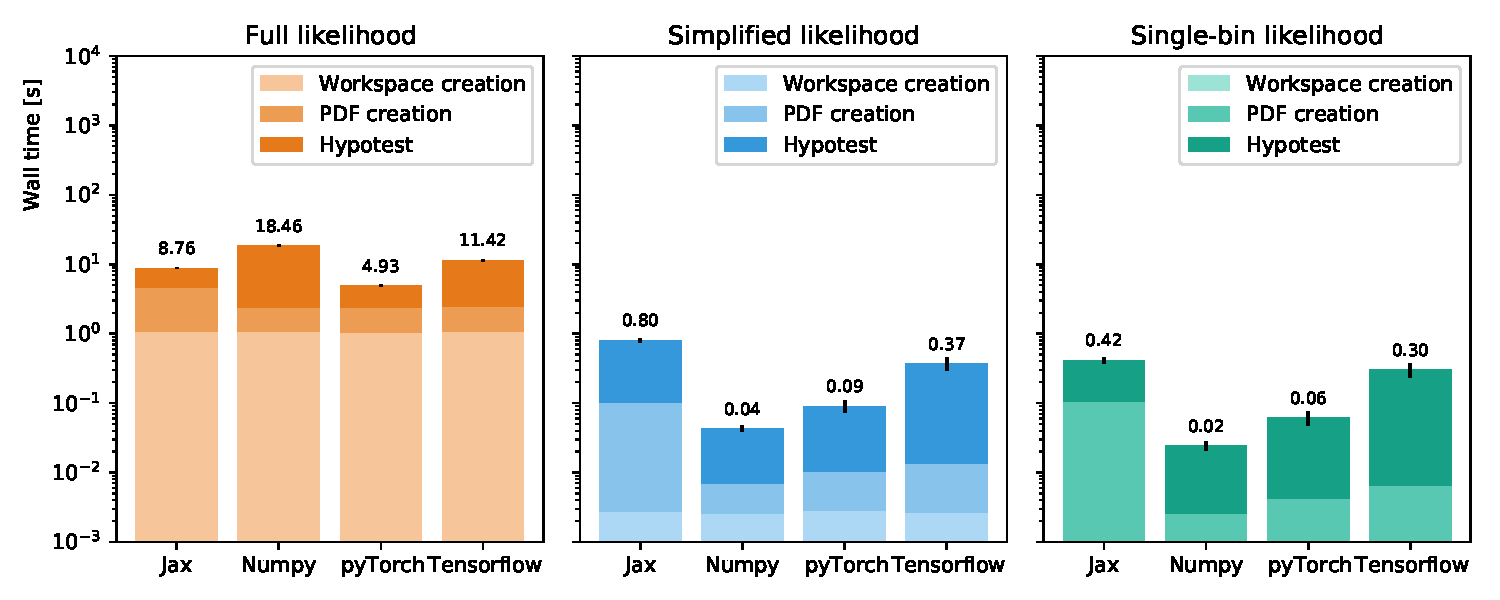
\includegraphics[width=\textwidth]{benchmark_1Lbb}
	\caption{Benchmarks of the CPU-time necessary for hypothesis testing using different likelihood and \texttt{pyhf} configurations in the context of the ATLAS 1L electroweakino search, run on a non-isolated CPU with 4 threads. The full likelihood (left) includes the full statistical implementation of the original analysis, the simplified likelihood (center) represents the simplified likelihood approach presented in this document, and the single-bin likelihood (right) represents a single-bin approximation of the ATLAS 1L electroweakino search. The uncertainties represent the standard deviation of the benchmark test sample.}\label{fig:benchmark}
	\label{fig:benchmark_1Lbb}
\end{figure}


\section{Physics performance}\label{sec:physics_performance}